%File: formatting-instruction.tex
\documentclass[letterpaper]{article}
\usepackage{aaai}
\usepackage{times}
\usepackage{helvet}
\usepackage{courier}
\usepackage{url}
\usepackage{graphicx}
\usepackage{amsmath}
\usepackage{latexsym}
\usepackage{amssymb}
\usepackage{multirow}
\newtheorem{definition}{Definition}
\frenchspacing
\setlength{\pdfpagewidth}{8.5in}
\setlength{\pdfpageheight}{11in}
\pdfinfo{
/Title (Insert Your Title Here)
/Author (Put All Your Authors Here, Separated by Commas)}
\setcounter{secnumdepth}{0}  
 \begin{document}
% The file aaai.sty is the style file for AAAI Press 
% proceedings, working notes, and technical reports.
%
\title{Resonation Elicits Diffusion: \\Modelling Subjectivity for Retweeting Analysis}
%\author{AAAI Press\\
%Association for the Advancement of Artificial Intelligence\\
%2275 East Bayshore Road, Suite 160\\
%Palo Alto, California 94303\\
%}
\maketitle
\begin{abstract}
\begin{quote}
Retweeting is the core mechanism of information diffusion on Twitter. User modelling has been proved effective in  retweeting behavior analysis, however none studies have investigated the subjectivity of users. 
In this paper, we propose a subjective model by combining both topics of interest and opinions to model users, and demonstrate that a user is more likely to retweet a message because of subjective similarity. 
We define a novel weighting function to measure the subjective similarity. 
By means of ANOVA test, the subjective similarity is verified to be correlated with  retweeting behavior;  
we compare our model with other content-based models in retweeting prediction and results show that our model  outperforms other models for predicting retweeting behavior; 
when combining with other factors, subjective similarities give significant improvement over a off-the-shelf predicting model.
\end{quote}
\end{abstract}

\section{Introduction}
\label{introduction}
\noindent Microblogging has become a center of attention in the area of social networking due to the amount of users it has attracted and the volume of messages it produces daily. 
Microblogging services such as Twitter appear to play an important role in the process of information dissemination on the Internet, making it possible for messages to spread virally in a matter of minutes. 
Retweeting convention and complex network of Twitter provide an unprecedented mechanism for the spread of information despite the restricted length of a single message(tweet) \cite{Jenders:2013APV}. 
Actually almost a quarter of the tweets are retweeted from others \cite{conf/cikm/YangGCTLZS10}. 
Understanding how retweeting behavior works can help explaining information dissemination on Twitter. 

Studies have tried to find factors that influence whether a tweet will be retweeted \cite{Boyd2010,Kwak:2010TSN,Suh2010}. 
Users receive thousands of tweets on different topics every day, whether a tweet will be retweeted will depend on the subjective choice of users. 
From the point of a user, retweeting is a process that includes reading the tweet, estimating the content and deciding to share. The crucial part is to estimate whether a tweet contains information interesting to the user who might find it worthy to be shared.  
Therefore modelling the motivation of users provides an important perspective for retweeting behavior analysis. 
This research is motivated by a desire to understand what drives users of social networks to disseminate information they come across. 

Previous studies on retweeting behavior have shown that an enriched user model gives coherent and consistent explanation for retweeting motivation \cite{conf/icwsm/MacskassyM11,conf/wsdm/FengW13}. 
Specifically, researchers have tried to model users from four types of information:
profile features (``\textbf{Who you are}"), tweeting behavior (``\textbf{How you tweet}"), linguistic content (``\textbf{What you tweet}") and social network (``\textbf{Who you tweet}") \cite{Pennacchiotti:icwsm11}. 
Subjective initiative nature of human determines that his behavior pattern is subjectivity driven. 
According to theory of Biased Assimilation, people are prone to choose and disseminate information according to their own biased subjectivity \cite{Hyman2000}. 
Therefore, we can understand the underlying reason why a user retweet a message by modelling the subjectivity of the user. 

Twitter has become a platform where different opinions are presented and exchanged by allowing users publish subjective messages on topics they are interested in. 
Therefore subjectivity of a user is encoded in the millions of User-Generated Content(UGC) on Twitter. 
In this study we explore the big text data with state-of-the-art Natural Language Processing techniques to model the subjectivity of users, and investigate whether the subjective model could benefit the retweeting behavior analysis. 
Intuitively, we put forwards that subjectivity can be represented as topics and opinions articulated in the tweets generated by users on Twitter. 
And the probabilty a user retweets a message could be evaluated by measuring the subjective similarity between the tweet and the subjective model of the user. 

\section{Subjective Model}
\label{subjectivemodel}

Subjectivity has been extensively studied by psychologists to characterize the personality of a person based on his historic behaviors and remarks \cite{Engbert2007}. 
Linguists define the subjectivity of language as speakers always show their perspectives, attitudes and sentiments to events, people, topics, and entities in their languistic content \cite{stein2005subjectivity}. 
How to computationally model subjectivity of a user is still a challenging problem for many applications. 
The advent of online social networking such as Twitter has given a new layout to the challenge.  
Twitter allows users to show their personal subjectivity by publishing short messages, which give researchers resources to model the subjectivity of users.
First of all, we give an formal definition for subjective model under context of Twitter.

\subsection{Definition}
\label{definition}

Let $G=\left( V,E \right) $ denotes a social network, where $ V $ is a set of users on Twitter, and $ E\subset V\times V $ is a set of directed relationships between users. For each user $ u \in V $, there is a tweets collection $ M_{u} $ denotes his message history. We assume there is a topic space $ T $ containing all topics they talk about, and a sentiment valence space $ O $ for evaluating their opinions towards these topics. 
For the ``subjectivity'' of a user $ u $, we refer to both topics of interest and opinions articulated in his tweets collection $ M_{u} $.  
\begin{definition}[Subjective Model]
The subjective model $ P \left( u \right) $ of a user $u \in V $, is the combination of a set of topics $\left\lbrace  t_{i} \left( i \in \lbrace1 \cdots n \rbrace \right)  \right\rbrace $ the user talks about in a topic space $T$ and the user's opinion $o_{i}$ towards each topic $ t_{i} $. 
\begin{equation}
\label{usermodel}
P \left( u \right) = \lbrace \left( t_{i}, w_{u} \left( t_{i} \right), d_{u,t_{i}} \left( o_{i} \right) \right) \,\vert  t_{i} \in T, \, o_{i} \in O \rbrace
\end{equation}
where:
\begin{itemize}
\item with respect to the given user $ u $,  for each topic $t_{i} \in T$, its  weight $ w_{u} \left( t_{i} \right)$ represents the distribution of the user's interests on it, with $ \sum_{i=1}^{|T|}w_{u} \left( t_{i} \right)=1 $.
\item opinion of the user towards topic $t_{i}$ is modeled as a topic-dependent sentiment distribution  $d_{u,t_{i}} \left( o_{i} \right)$ over sentiment valence space $ O $.
\end{itemize}
\end{definition}
The definition of subjective model given above is in an abstract form by using latent concepts of topics and opinions,  which need to be derived from message history of all users $ M=\lbrace M_{u}\vert u \in V\rbrace$  

\subsection{Establishment of Subjective Model}
\label{establishment}
According to the definition, subjective model of a user can be represented as two distributions: the topic distribution and the sentiment distribution for each topic. 
With state-of-the-art topic model and sentiment analysis techniques, we can establish subjective model by finding topics and opinions simultaneously. 
\subsubsection{Topic Analysis}
\label{topic}
Previous studies have tried to identify topics by finding key words \cite{Chen:2010STE}, extracting  entities \cite{Abel:2011AUM} or linking tweets to external knowledge categories \cite{conf/icwsm/MacskassyM11}. Recent works show that topic models such as \textbf{Latent Dirichlet Allocation (LDA)} model \cite{blei2003latent} have been efficient ways to characterize latent topics of large volume corpus.  
Topics of LDA are broader in concept, since a single topic consists of the whole collection of related words, so we adopt the LDA topic model for topic analysis.  
Topic analysis for all users in a global network on Twitter is a nontrivial task. 
There are millions of users and billions of tweets associcated with these users, and the effectiveness and efficiency of topic model is a big problem.
However, the ``following'' relationship on Twitter is a strong indicator of a phenomenon called ``homophily", which has been observed in many social networks \cite{mcpherson2001birds}.
Homophily implies that a user follows another user because of sharing common topics of interest. 
According to the principle of homophily, we put forwards the concept of \textbf{Local Topic Space}: 
\begin{definition}[Local Topic Space]
\label{local}
Let $G=\left( V,E \right) $ denotes a global social network, for a user $ u \in V $, we use $ G_{u}^{\tau} \subseteq G$ 
to denote $ u $'s $ \tau $-ego network, where $ \tau $ -ego network means a subnetwork formed by $ u $'s $ \tau $-hop 
friends in the network $ G $, and $ \tau \geqslant 1 $ is a tunable integer parameter to control the scale of the ego network. 
In the $ \tau $-ego network of user $ u $, all users concentrate on a few topics derived from the content generated by them, and these topics form a local topic space $ T_{u} $.
\end{definition}
The relatively tiny size and topic homophily of ego network lower the impact of data sparsity and degrade the complexity of calculation.

Therefore we adopt a user-level LDA model to find latent topics in Local Topic Space by aggregating all tweets generated by a user into a single document just as \cite{Hong:2010EST}. 
The result of LDA produces two multinomial distributions, with distribution $ \theta_{u} $ representing the probability distribution of a user over each topic, and distribution $ \beta_{k} $ representing the probability distribution of a topic over whole vocabulary used by all users in ego network. 

\subsubsection{Opinion Analysis}
\label{opinion}

Users often express opinions towards topics of interest by publishing topic-related tweets. 
Sentiment analysis or opinion mining is formally defined as the computational study of sentiments and opinions about topics expressed in a text \cite{liu2012sentiment}. Opinions are regulated as sequential discrete values to represent sentiment strength(for example: 0 stands for negtive and 1 for positive). Recently, researchers began to pay more and more attention to social media such as Twitter \cite{Thelwall:2010SSS,Thelwall:2012SSD,Hu:2013www} and provide effective sentiment analysis tools. 

SentiStrength package has been built especially to cope with sentiment analysis in short informal text of social media \cite{Thelwall:2010SSS}. 
It combines lexicon-based approaches with sophisticated linguistic rules adapted to social media, which is suitable for analyzing sentiment of tweets.
SentiStrength assigns two values to each tweet standing for sentiment strengths: a positive and a negative sentiment measurement, with $ \left[ -5,-1 \right]  $ denoting negative and $ \left[ 1,5 \right]  $ denoting positive sentiment strength.
Sentiment assigned by SentiStrength is a fine-grained strength, which can catch fine opinion distributions in a user's subjective model.  
For the convenience of distribution calculation, we map the output of SentiStrength to single-scaled sentiment valence space $ \left[ 0, 8 \right] $ as follows:
\begin{equation}
\label{opinionmap}
o= \left\{ 
\begin{array}{lll}
{p+3} & if \vert p \vert > \vert n \vert \\
{n+5} & \text{if } \vert n \vert > \vert p \vert \\
{4}  & \text{if } \vert p \vert = \vert n \vert
\end{array}
\right.
\end{equation}
Where $ p $ denotes the positive setiment strength and $ n $ denotes negative sentment strength.
In the sentiment valence space, value 4 indicates neutral sentiment, while values above 4 indicate positive sentiment and values below 4 indicate negative sentiment. 

\subsubsection{Concrete Subjective Model}
\label{concrete}
 
As Definition~\ref{local} describes, for a user $ u $ in a global netwotk, we can extract a $ \tau $-ego network $ G_{u}=\left( U,E_{u} \right)  $. 
And the subjective model of each user $ u \in G_{u} $ can be concreted within the ego network. 
We denote tweets set published by a user $ u $ as $ M_{u}=\left\lbrace m_{i} \vert i \in \left[ 1, \cdots, N \right]  \right\rbrace$. All tweets in $ M_{u} $ is concatenated to a single document $ d_{u} $ to construct Local Topic Space $ T_{u}=\left\lbrace t_{i} \vert i=1, \cdots, K \right\rbrace $ with LDA topic model.
The topic model is built with parameter $ \theta_{u} $\ representing the distribution of user $ u $ over topics he talks about, and parameter $ \beta_{k} $ represents the distribution of each topic over the vocabulary of all tweets. SentiStrength is applied to each tweet $ m $ in collection $ M_{u} $ and outputs sentiment strength $ s_{m} $ for tweet $ m $. 
Subjective model of user $ u $ is built the  as follows:
\begin{itemize}
\item Firstly, for user $ u $, the corresponding $ \theta_{u} $ can be regarded as his topic distribution in the Local Topic Space $ T_{u} $, and topics he cares about are $ Z_{u}= \left\lbrace z \vert p\left( z \vert \theta_{u}\left( z \right)  \right)>0 \right\rbrace $.
\item Secondly, in order to identify the target of opinion in each tweet, the topic model is applied to each tweet $ m $ to find topics it talks about, which are $ Z_{m} =\left\lbrace z_{m} \vert p\left( z_{m} \vert \theta, \beta, Z_{u} \right)>0 \right\rbrace $.
\item Thirdly, the opinion distribution of user $ u $ towards topic $ t \in Z_{u} $ could be calculated as: 
\begin{equation}
\label{opinionall}
d_{u,t}\left( o \right) = \left\lbrace \dfrac{N_{o}}{\sum_{o \in O} N_{o}} \vert O=\left[ 0, \cdots, 8 \right] \right\rbrace 
\end{equation}
where $ N_{o} $ is the number of times user $ u $ expresses an opinion towards topic $ t $ with sentiment strength $ o $, which could be calculated as:
\begin{equation}
\label{opinion1}
N_{o}=\sum_{m \in Mu} I\left( s_{m} \right) , \text{ if } s_{m}=o \& t \in Z_{m}
\end{equation}
\begin{equation}
\label{opinion2}
I\left( s_{m} \right)=\left\{
\begin{array}{ll}
{1} & \text{if } s_{m}=o \& t \in Z_{m}\\
{0} & \text{else}
\end{array}
\right.
\end{equation}
where $ s_{m} $ denotes the sentiment strength of tweet $ m $. For simplicity, we assume the sentiment of tweet $ m $ is related to every topic it talks about in $ Z_{m} $.
\end{itemize}

Totally, we build subjective model $ P\left( u \right) $ for user $ u $ as:
\begin{equation}
\label{subuser}
P\left( u \right)= \left\lbrace \left( t, p\left( z \vert \theta_{u} \right), d_{u,t}\left( o \right) \right)  \vert t \in Z_{u}, o \in O  \right\rbrace  
\end{equation}

\section{Retweeting Analysis With Subjective Model}

Many factors have been proved to influence retweeting behavior \cite{Suh2010,conf/icwsm/MacskassyM11,Comarela:2012UFA}, however few researches have investigated the subjective motivation of a user to retweet a message. 
Therefore we will study whether subjective model can help understand underlying reasons of a user's retweeting behavior.
Apart from the context constraints, a tweet is more likely to be retweeted by subjective users who find it worth to. 
Therefore, we are not interested in modelling the tweet by itself as other researches \cite{Naveed:2011SMC,2011:NaveedGKC,conf/icwsm/PfitznerGS12}, but how the tweet resonate with the users who might want to disseminate it. 
We assume the motivation of a user to retweet a message lies in that the user considers only the tweet content arousing his resonation without context perturbation. 
If a tweet is published, all followers of its author will receive it in time, and followers are likely to retweet it if they find it worthwhile. 
Under such assumption, we investigate the problem in 1-ego network for the author of target tweet. 
The relation between tweet, author and followers can be illustrated as Figure~\ref{fig1}.
\begin{figure}[htb]
%\setlength{\belowcaptionskip}{-0.2cm} 
\centering
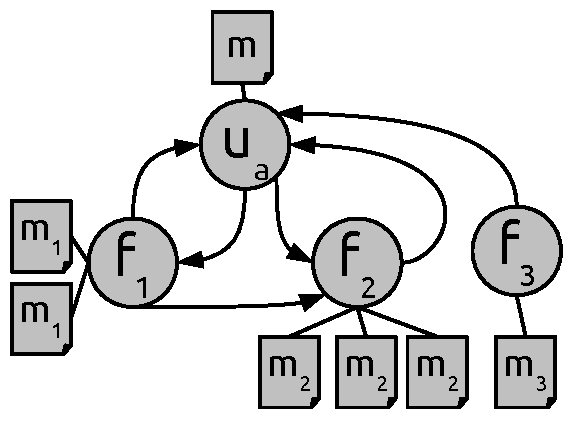
\includegraphics[width=2.1in,height=2.0in]{ego.pdf}
%\vspace{-4em}
\caption{Illustration of relations between tweet, author and followers. Author is denoted as $ u_{a} $, tweet as $ m $, followers as $ f_{i} $ and tweets of follower $ f_{i} $ as $ m_{i} $. An directed edge $ \left( f_{i},u_{a} \right)  $ means that $ f_{i} $ is exposed to the messages published by $ u_{a} $.}
\label{fig1}
\end{figure}

\subsection{Problem Formulation}
\label{formulation}

Retweeting analysis problem can be formulated as follows:
For each target tweet $ m $, let $ F $ denotes the followers who receive $ m $ by following its author $ u_{a} $, and for each user $ u \in F \cup \left\lbrace u_{a} \right\rbrace  $, let $ M_{u} $ denotes   tweets the user has published. 
For each follower $ u_{f} \in F $, we can define a quadruple $ <u_{f}, u_{a}, m, r_{f}>  $: 
\begin{itemize}
\item $ r_{f} $ is a binary label indicating whether $ m $ is retweeted by $ u_{f} $.
\item Firstly our work focuses on building subjective model $ P\left( u \right)  $ for each user $ u \in F \cup \left\lbrace u_{a} \right\rbrace $ in the ego network with all tweets collections $ M=\left\lbrace M_{u} | u \in F \cup \left\lbrace u_{a} \right\rbrace  \right\rbrace  $.
\item Then we investigate the relation between the subjectivity of a user and his retweeting behavior to predict $ r_{f} $ by calculating subjective similarities between tweet $ m $, its author $ u_{a} $ and follower $ u_{f} $. 
\end{itemize}

\subsection{Subjective Similarity}
\label{similarity}

In order o understand the underlying reasons why a user retweet a message, we try to simulate the subjective decision-making procedure by investigating the relationship among a tweets and subjective models of its author and followers. 
We assume that if a tweet and the subjective models of a user are similar enough in terms of topics and opinions, the user will have a very high probability to retweet the tweet. 
We call this phenomenon as ``resonation'', and assume resonation between tweets and users will elicit retweeting behavior.
With subjective models built for users, we can define a similarity measurement to quantify the resonation among them.

\subsubsection{Topic Similarity}
\label{topsim}

Topic distribution of a tweet can be inferenced by applying topic model estimated from the tweets collections of users.
The topic similarity between tweet and user can be calculated with methods such as the cosine distance \cite{cha2007comprehensive} or the Jensen-Shannon Divergence \cite{weng2010twitterrank} with satisfactory results.
In our research, we adopt cosine distance to measure the topic similarity, which is defined as:
\begin{equation}
sim_{topic}=\dfrac{\theta_{m} \cdot \theta_{u}}{\parallel \theta_{m} \parallel \parallel \theta_{u} \parallel}
\end{equation}
where $ \theta_{u}$ denotes topic distribution of user $ u $ and $\theta_{m}$ denotes topic distribution of tweet $ m $. 

\subsubsection{Opinion Similarity}
\label{opsim}

Opinions of a tweet can be analyzed with SenStrength and the values are transformed to range $ \left[ 0,8 \right]  $  with Equation~\ref{opinionmap}.
Opinions of a tweet towards each topic it talks about can be regarded as a distribution with 1.0 probability on a single sentiment value just as opinion dsitribution of subjective model. 
Therefore opinion similarity between tweets and users is the same with similarity between two users.   
We treate opinion as distribution over sentiment valence space with each element of the distribution represents the propotion of the corresponding strength values in the user's all sentiment values. 
However ,values in sentiment valence space are not independent. 
They are sequential and represent strength of the sentiment, for example value 8 represents more positive sentiment than value 5, and their sentiment distance is 3.
Therefore, opinion similarity can not be calculated as the distance between two distributions.
Illustrated as Table~\ref{tab1}, $ user_{1} $ holds most negative opinion on a topic(with 100\% sentiment value 0), while $ user_{2} $(100\% positive sentiment value 7) and $ user_{3} $(100\% positive sentiment value 8) hold positive opinion.
If cosine similarity measurement is adopted to calculate opinion similarity, all similarities are 0.
In fact $ user_{2} $ is more similar with $ user_{3} $ than $ user_{1} $ because they both hold positive opinion and their sentiment distance is much less than $ user_{1} $. 
\begin{table}[h]
\scriptsize
\centering
\caption{Illustration of opinion similarity calculation}
\label{tab1}
\begin{tabular}{|l|l|l|l|l|l|l|l|l|l|}
\hline
 & 0 & 1& 2 & 3 & 4 & 5 & 6 & 7 & 8 \\
\hline
$user_{1}$ & 1.0 & 0.0 & 0.0 & 0.0 & 0.0 & 0.0 & 0.0 & 0.0 & 0.0 \\
\hline
$user_{2}$ & 0.0 & 0.0 & 0.0 & 0.0 & 0.0 & 0.0 & 0.0 & 1.0 & 0.0 \\
\hline
$user_{3}$ & 0.0 & 0.0 & 0.0 & 0.0 & 0.0 & 0.0 & 0.0 & 0.0 & 1.0 \\
\hline
\end{tabular}
\end{table}  
In order to accurately catch opinion similarity, we propose a novel similarity-calculating method by combining both sentiment distance and distribution similarity.
The opinion similarity of two users or a tweet and a user on topic $ t $ can be calculated as: 
\begin{equation}
sim_{opinion}^{t}(O_{1},O_{2})=\dfrac{8-|\sum_{i=0}^{8}d_{i}v_{i}-\sum_{j=0}^{8}d_{j}v_{j}|}{8}
\end{equation}
where $ d_{i} $ denotes the $ ith $ distribution of opinion vector, and $ v_{i} $ denotes corresponding sentiment strength value.
Accordingly, overall opinion similarity on all topics can be calculated as normalized similarity of all opinion similarities on their common topics of interest. 
\begin{equation}
sim_{opinion}(u_{1},u_{2})=\dfrac{\sum_{t=1}^{|T|}sim_{opinion}^{t}(O_{1},O_{2})}{|T|}
\end{equation}
where $ T $ denotes the common topics of interest between two users or a tweet and a user.

\subsubsection{Subjective Similarity}

Given a tweet $ t $ and a user subjective model $ P\left( u \right)  $, we can define their subjective similarity by combining topic similarity and opinion similarity as follows:
\begin{equation}
Sim_{sub} \left( t,u \right) = \alpha * sim_{topic}+\left( 1-\alpha \right)*sim_{opinion}
\end{equation}
where $ \alpha $ is the coefficient used to control the proportions of topic similarity and opinion similarity in the holistic subjective similarity. 
A user cares more about topics a tweet talks about with a larger $ \alpha $, and cares more about opinions with a samller $ \alpha $. 
A personalized $ \alpha $ can be learned from the retweeting history of a user to represent his retweeting habit. 

\subsection{Retweeting Analysis}
\label{analysis}
The motivation why a user retweet is complicated, and involves the tweet itself, its author and its receivers who is following its author. 
Figure~\ref{fig1} illustrates their relation. 
The idea behind this work is that taking into account user attitudes towards his own interests can yield benefits in explaining the subjective motivation of retweeting behavior. 
Specifically, we consider this question from three aspects: 
(i) how similar is the tweet to the subjective model of a user in terms of topics and opinions, i.e. $ sim_{sub} \left( m,u \right) $, (ii) are the author and user like-minded people considering similarity of their subjective models, i.e. $ sim_{sub}\left( u_{a},u \right)  $, and (iii) whether the tweet is novel or original judged from its similarity with subjective model of its author, i.e. $ sim_{sub}\left( m,u_{a} \right)  $. 
Intuitionally, a user might retweet a message if its content is close enough to his subjectivity, its author is a like-minded friend and it is original from inner subjectivity of its author. 
In this work we will carry out a sery of experiments to demonstrate such intuition.

\section{Experiment}
\label{experiment}

\subsection{Dataset}
We adopt the Twitter dataset of previous work \cite{Luo:2013RMF}, which was created using Twitter API \footnote{\url{https://dev.twitter.com/}}. 
To form the dataset, 500 target English tweets published from September 14th, 2012 to October 1st, 2012 were monitored to find who would retweet it in the next few days. 
And each tweet was chosen as starting point to collect at least recent 200 tweets for its author and followers.
Overall, there are 4,5531 followers, 6,277,736 tweets, and 5214 followers who have retweeted at least one target tweet during the monitored period. 
We extract 3,0876 users who have retweeted at least 20 times in their recent tweets to build their sujective model and study their retweeting motivations. 
In order to determine the optimized values of $ \alpha $ in subjective similarities($ sim_{sub} \left( m,u \right) $, $ sim_{sub}\left( u_{a},u \right)  $, $ sim_{sub}\left( m,u_{a} \right)  $), we implemented a \textit{mini-batch gradient descent} algorithm with the users' retweeting history. As a result, all three subjective similarities are optimized to reflect the personalized retweeting habits of each users.

\subsection{Correlation of Subjectivity and Retweeting Behavior}

The first step of demonstrating our intuition is to assessing the existence of a correlation between subjective similarity and retweeting behaviour. 
To test this correlation, we adopt a statistical hypothesis test called Analysis of Variance (ANOVA). 
ANOVA tests the \textit{null hypothesis} that samples in two or more groups are derived from the same population by estimating the variance of their means. This test fits our goal of testing if the distinct sets of retweeters and non-retweeters do have the same subjective similarity to a tweet that both sets are exposed to. 
The ANOVA method produces two output values: the \textit{F-ratio} and the \textit{p-value}. 
If the difference between the means is due to chance, the expected value of the \textit{F-ratio} is 1.00. 
If ANOVA yields a p-value lower than the significance level $ \alpha $, the \textit{null hypothesis} is rejected. 
The significance level is conventionally used at 0.01.
At the same time, we carry out the test by varying the number of topics in LDA as 50, 100 , 150 and 200 to determine impact of topic number. 
The results are listed in Table~\ref{tab2}, 
\begin{table}[h]
\scriptsize
\centering
\caption{ANOVA test for three subjective similarities}
\label{tab2}
\begin{tabular}{|c|c|c|c|c|}
\hline
\multicolumn{2}{|c|}{Similarity}& $ sim_{sub} \left( m,u \right) $ & $ sim_{sub}\left( u_{a},u \right)  $ & $ sim_{sub}\left( m,u_{a} \right)  $\\
\hline
\multirow{2}{*}{50} & \textit{F} & \textbf{12.182} & 2.212 & 4.236 \\
\cline{2-5}
  & \textit{p} &  $\mathbf{4.44e^{-06}}$  & 0.140 & 0.272\\
\hline
\multirow{2}{*}{100} & \textit{F} & \textbf{22.356} & \textbf{12.240} & \textbf{14.664} \\
\cline{2-5}
  & \textit{p} &  $\mathbf{2.43e^{-08}}$  & $\mathbf{6.25e^{-06}}$ & $\mathbf{8.46e^{-07}}$\\
\hline
\multirow{2}{*}{150} & \textit{F} & \textbf{43.892} & \textbf{31.145} & \textbf{28.466} \\
\cline{2-5}
  & \textit{p} &  $\mathbf{8.65e^{-11}}$  & $\mathbf{3.55e^{-08}}$ & $\mathbf{1.32e^{-09}}$\\
\hline
\multirow{2}{*}{200} & \textit{F} & \textbf{31.675} & \textbf{20.616} & 6.145\\
\cline{2-5}
  & \textit{p} &  $\mathbf{4.22e^{-06}}$  & $\mathbf{2.92e^{-05}}$ & 0.26\\
\hline
\end{tabular}
\end{table}

Note that for the number of topics 100 and 150, all similarities yield \textit{p-values} below $ \alpha $. This suggests that subjective similarities can be good indicators for modeling retweeting behavior. 
Therefore we reject the \textit{null hypothesis} and accept the alternative hypothesis.
For the rest experiments, we simply set the number of topic as 100 for LDA. 

\subsection{Comparison With Other Models}
\label{Comparison}

Given that ANOVA indicated correlation between subjective similarities and retweeting behavior, we compare three similarities against other content-based similarity measurements such as TF-IDF model(modelling user with bag-of-words in his tweets) \cite{Luo:2013RMF}, entity-based model(model user with entities extracted from his tweets) and hashtag-based model(model user with hashtags used in his tweets) \cite{Abel:2011AUM}.

We take 5,214 retweeters in our dataset who retweet at least one target tweet as positive instances, and randomly sample 5,214 negative instances from the 40,317 followers who do not retweet any target tweet.
The balance dataset of all positive and negative instances is randomly divided into five parts for 5-fold cross-validation. 
We use the logistic regression classifier of Scikit-learn machine learning package \cite{scikit-learn} for training and testing.
Accuracy is our evaluation metric, and the result is listed in Table~\ref{tab3}.
\begin{table}[h]
\centering
\caption{Comparison of prediction accuracy for different models. }
\label{tab3}
\begin{tabular}{|c|c|}
\hline
Feature & Accuracy(\%) \\
\hline
TF-IDF & 60.85  \\
entity & 68.76 \\
hashtag & 59.12  \\
$ sim_{sub} \left( m,u \right) $ & 73.88\\
$ sim_{sub}\left( u_{a},u \right)  $ & 70.04\\
$ sim_{sub}\left( m,u_{a} \right)  $ &69.64\\
$ sim_{all}  $ &\textbf{75.64}\\
\hline
\end{tabular}
\end{table}

The best accuracy(75.64\%) is achieved by the $ sim_{all}  $, for which We put all three subjective similarities into classifier to test impact of their combination.
The perfromance of TF-IDF model(60.85\%) is moderate.  
Entity-based model(68.76\%) is very close to  $ sim_{sub}\left( u_{a},u \right)$(70.04\%) and $ sim_{sub}\left( m,u_{a} \right)  $(69.64\%), and their difference is not significant.
While for hashtag-based model, its accuracy is the lowest(59.12\%), the reason might lie in a very low usage of hashtag in users' tweets. 
The performance of $ sim_{sub} \left( m,u \right) $(73.88\%) is better than others except for $ sim_{all}  $.
The results above show that subjective model can better help understand retweeting behavior than other user models.

\subsubsection{Combining Evaluation With Other Factors}
\label{combining}
Subjective model tries to catch the subjective motivation of users based on their tweets content, whereas other important factors associated with retweeting behavior are not considered, such as network topology and metadata of the user, etc. 
In this section, we combine subjective similarities with other important factors that other researches have demonstrated. 
Firstly we compare the performance of our method with model of Luo \emph{et al.}~\shortcite{Luo:2013RMF}.
In their work they use four feature families: ``Retweet History''(follower who retweeted a user before is likely to retweet the user again), ``Follower Status''(the number of tweets, followers, friends, listed times and being verified), ``Follower Active Time''(interaction with others) and ``Follower Interests''(bag-of-words used to model users).
Secondly we demonstrate that performance of retweeting prediction could be improved significantly by using subjective model instead of bag-of-words model in their feature set. 
We use the same logistic regression classifier, dataset and settings as last experiment. The feature set of Luo \emph{et al.}~\shortcite{Luo:2013RMF} is marked as ``LUO''.
In addition, we set a baseline (marked as ``RB''), which simply predicts followers who have retweeted the author's previous tweets as retweeters of target tweet. 
The result is listed in Table~\ref{tab4}.
\begin{table}[h]
\centering
\caption{Prediction Accuracy of Different Models. Significant improvement over baseline with star($ \ast $) and LUO' model with dagger($ \ddagger $) (p$ < $0.05).}
\label{tab4}
\begin{tabular}{|l|l|}
\hline
Feature Set & Accuracy(\%) \\
\hline
RB & 60.85  \\
LUO & 71.76 $ \ast  $\\
$ sim_{sub} \left( m,u \right) $ & 73.88 $ \ast \quad \ddagger $\\
$ sim_{sub}\left( u_{a},u \right)  $ & 70.04 $ \ast  $\\
$ sim_{sub}\left( m,u_{a} \right)  $ &69.64 $ \ast  $\\
$ sim_{all}  $ & 75.64 $ \ast  \quad \ddagger $\\
LUO+$ sim_{sub} \left( m,u \right)$ & 74.04  $ \ast \quad \ddagger $ \\
LUO+$ sim_{sub}\left( u_{a},u \right)$ & 70.27  $ \ast $ \\
LUO+$ sim_{sub}\left( m,u_{a} \right)$ & 71.86  $ \ast $ \\
LUO+$ sim_{all}  $ & \textbf{78.15}  $ \ast \quad \ddagger $ \\
\hline
\end{tabular}
\end{table}

The accuracy of baseline is 60.85\%, and two prediction methods(``LUO'' and our model) both outperform the baseline significantly. 
$ sim_{sub} \left( m,u \right) $ and $ sim_{all}  $ outperform ``LUO'' significatantly.

After combining subjective similarities, the accuracy are changing. 
Noticing that, the most significant improvement(LUO+$ sim_{all}  $, 6.39\% improvement) is achieved by adding all three subjectivie similarities, which verifies our intuition. 
Subjective similarity between tweet and followers also gives significant improvement(LUO+$ sim_{sub} \left( m,u \right) $, 2.12\% improvement), which indicates that subjective resonation between tweet and followers can be considered as the underlying reason that elicits retweeting behavior. 
Adding other two subjective similarities can not improve performance significantly.

\subsection{Case Study}
\label{example}
In this section we give an vivid description about subjective model and its ability in explaining the retweeting behavior with an example. 
Topic and opinion of one target tweet, subjective models for its author, and two followers (one retweet it while the other does not) are shown as Figure~\ref{fig2}. 
The right part of each sub-figure illustrates topic distribution and the left part illustrates opinion distribution. 
It is clear that the tweet talks about the 14th topic of the local topic space. 
\begin{figure*}[htb]
%\setlength{\belowcaptionskip}{-0.2cm} 
\centering%,bb=0 0 1280 960
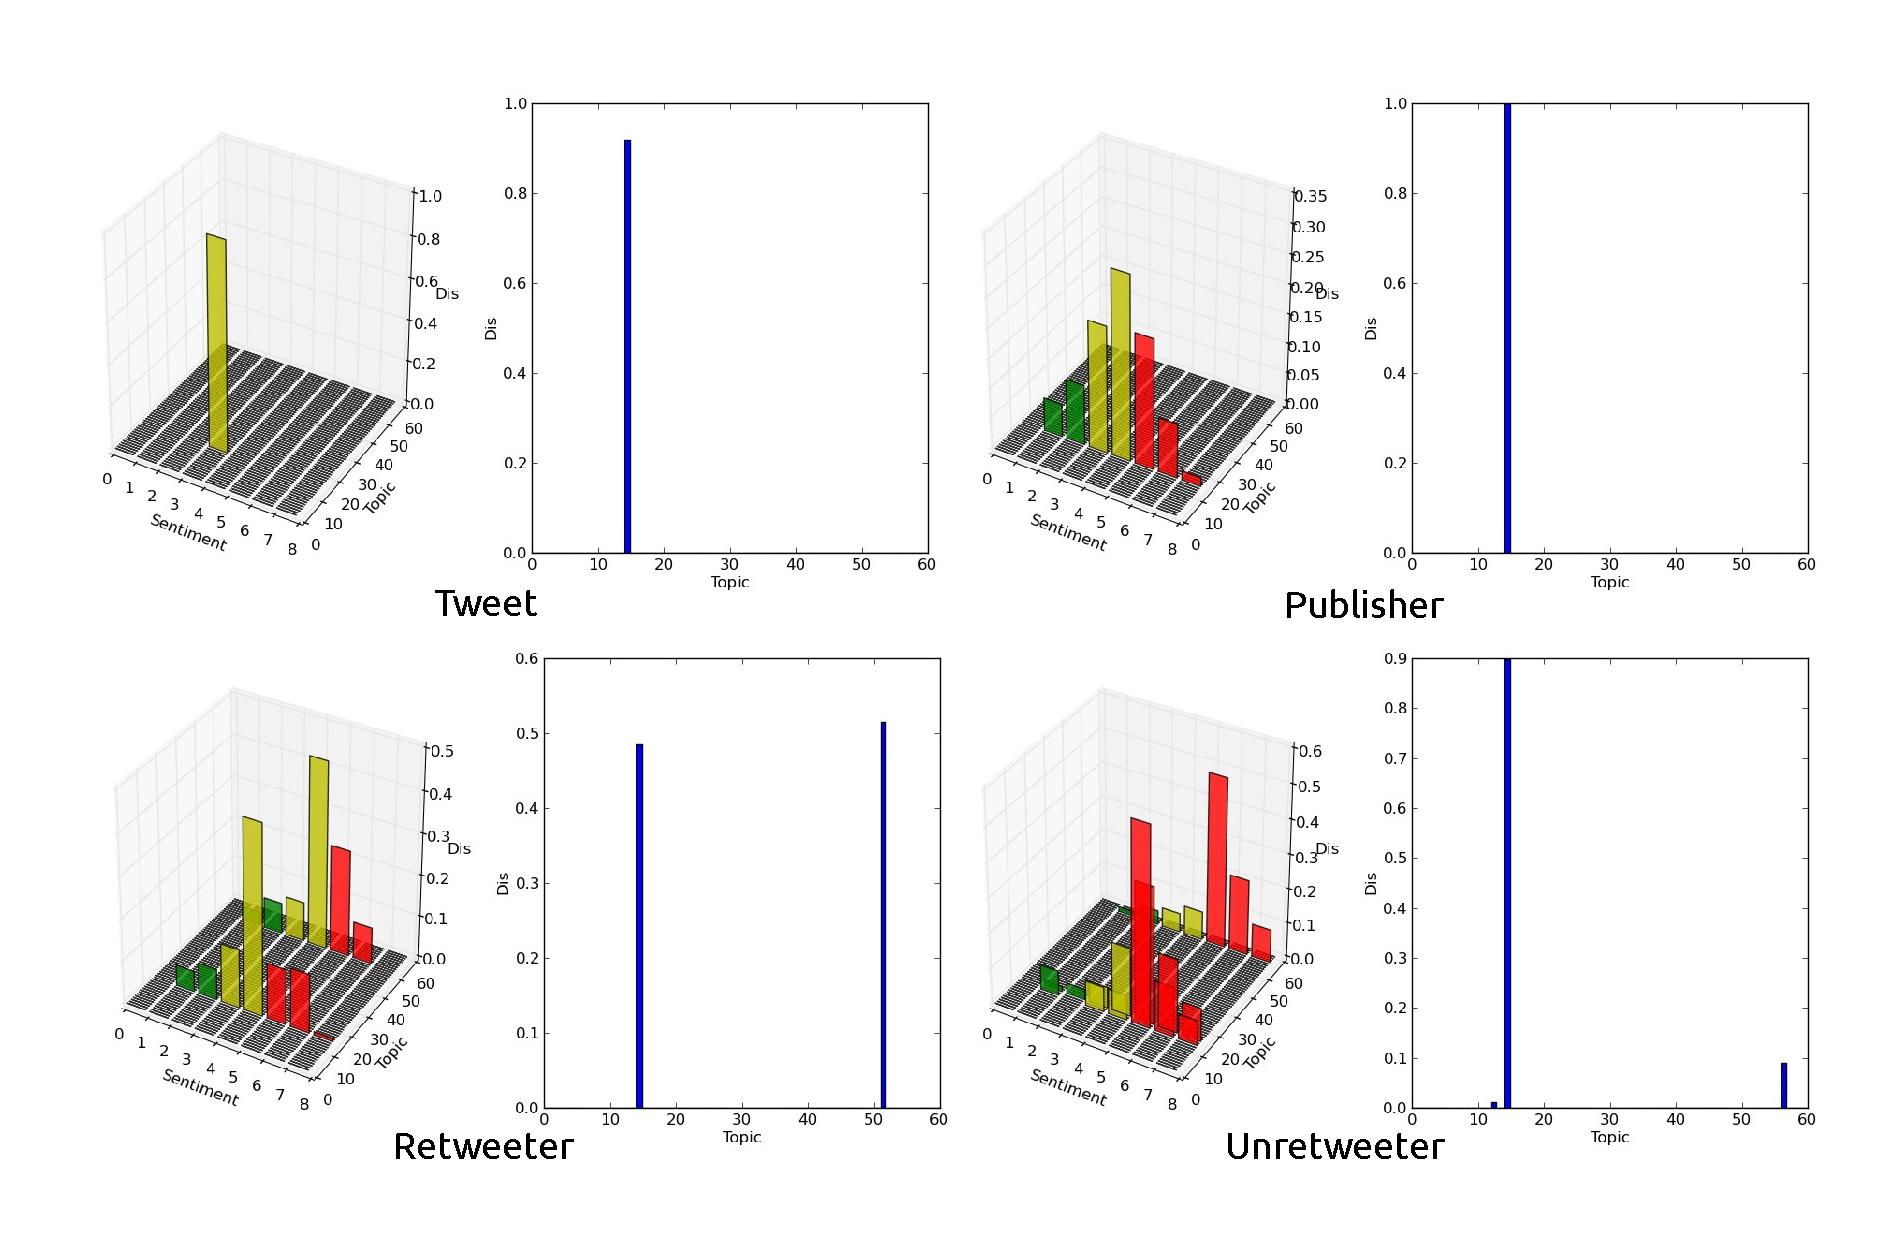
\includegraphics[width=6.0in,height=3.5in]{tweets10.pdf}
%\vspace{-4em}
\caption{Subjective model examples.}
\label{fig2}
\end{figure*}
Figure~\ref{fig3} shows top words of the 14th topic, the tweets of author and followers with word cloud\footnote{We use TagCrowd (\url{http://tagcrowd.com/}) to produce word cloud.}.
\begin{figure}[htb]
%\setlength{\belowcaptionskip}{-0.2cm} 
\centering
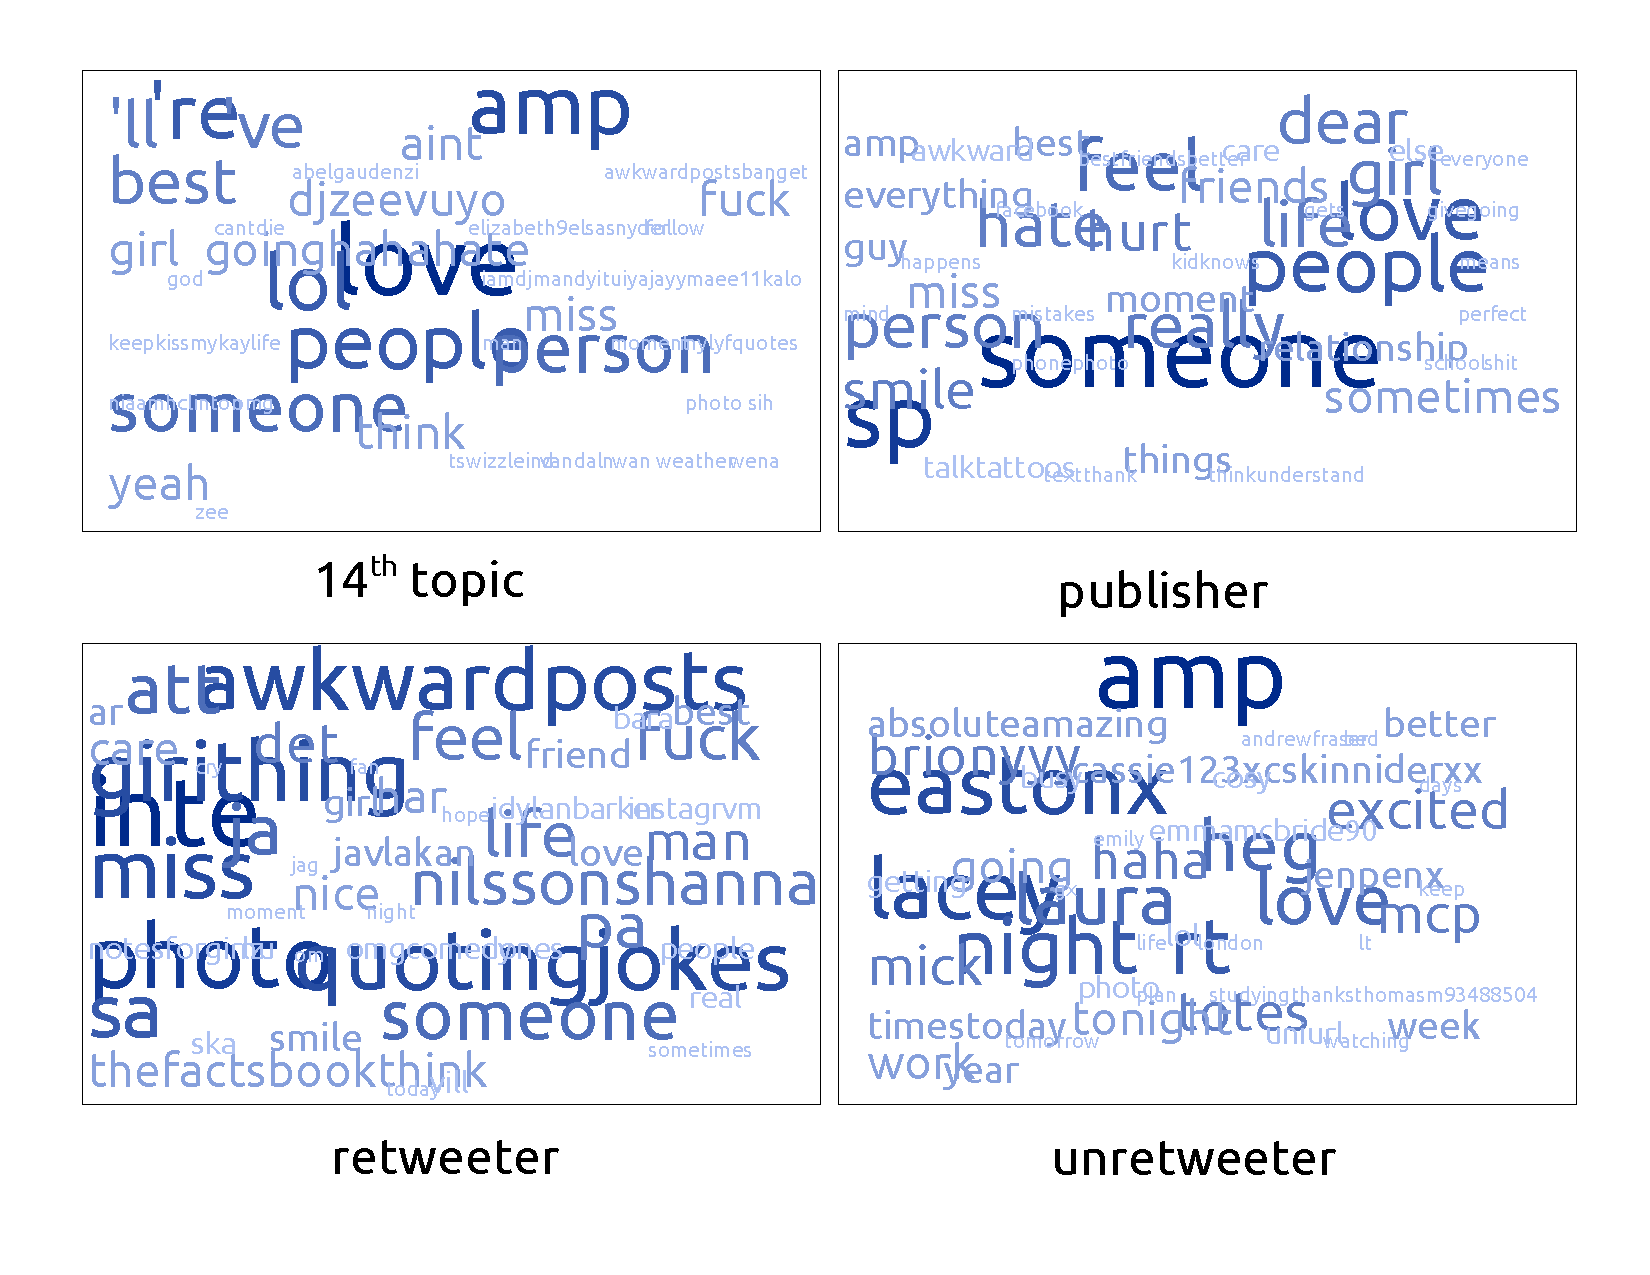
\includegraphics[width=3.5in,height=2.2in]{text_cloud.pdf}
%\vspace{-3em}
\caption{Word cloud of 14th topic, publisher and followers}
\label{fig3}
\end{figure}
Content of the tweet is:\\
\textit{Tweet: ``Sometimes the right person for you was there all along. You just didn’t see it because the wrong one was blocking the sight''} \\
The topic of this tweet is about ``love between people'' and the opinion is neutral, which is in accordance with the 14th topic word cloud in Figure~\ref{fig3} and sub-figure of tweet in Firgure~\ref{fig2}.
The author concentrates on the 14th topic, and his opinions are mainly neutral (as Figure~\ref{fig2},~\ref{fig3} show).
As for two followers, the ``retweeter'', has published tweets about two topics (the 14th and 52nd topic) uniformly and his opinions towards the two topics are mainly neutral.
While the ``unretweeter'', has also talked about two topics (14th and 56th topic), but he is mainly interested in 14th topic and has positive opinion.
Although two followers have same interest (the 14th topic), their different opinions elicit their different decision, which verifies subjective model can help better understand the retweeting motivation by modelling not only topics but opinions.

\section{Related Work}
\label{relatedwork}
   
User modelling provides researchers with insights into user's online behaviors. 
Hannon \emph{et al.}~\shortcite{Hannon:2010} proposed that Twitter users can be modeled by tweets content and the relation of Twitter social network, while content-based approach could find similar users who are "distant" without follow relations. 
Macskassy and Michelson~\shortcite{conf/icwsm/MacskassyM11} discover user's topics of interest by leveraging Wikipedia as external knowledge to determine a common set of high-level categories that covers entities in tweets. 
Ramage \emph{et al.}~\shortcite{RamageEtAl:10} made use of topic models to analyze Twitter content at the level of individual, showing improved performance on tasks such as post filtering and user recommendation. 
Xu \emph{et al.}~\shortcite{Xu:2012MUP} proposed a mixture model which incorporated three important factors, namely breaking news, friends' timeline and user interest, to explain user posting behavior.
Pennacchiotti and Popescu~\shortcite{Pennacchiotti:icwsm11} proposed a most comprehensive method to model Twitter user for user classification, confirming the value of in-depth features by exploiting the UGC.
A large body of studies have analyzed characteristics of retweeting \cite{conf/icwsm/MacskassyM11,Starbird:2012RRI}, examining factors that lead to increased retweetability \cite{Suh2010,Comarela:2012UFA} and designing models to estimate the probability of being retweeted \cite{Osborne_Lavrenko_2011,Jenders:2013APV,conf/icwsm/PfitznerGS12}.

\section{Conclusion}
In this paper, we propose subjective model to model users, and demostrate its ability in retweeting behavior analysis. We assume that retweeting should be elicited by the subjective similarities among the tweet and its author and followers. 
We define subjective model formally as the combination of topic distribution and opinion distribution, and we concrete subjective model leveraging statistical topic model and sentiment analysis techniques.
We demonstrate the effectiveness of our model for retweeting analysis problem and show that subjective model is able to reach better understanding of retweeting behavior. 

In the future, we will apply subjective model to other social network analysis task such as link prediction and friend recommendation. 

\bibliographystyle{aaai}
\bibliography{resonate_tweet}

\end{document}
